\documentclass[]{article}


\usepackage[margin=1cm,includehead,landscape]{geometry}
\usepackage{fancyhdr}
\usepackage{multicol}
\usepackage{graphicx}
\pagestyle{fancy}
\usepackage{amsmath}
\usepackage{amssymb}
\usepackage{float}
\usepackage{siunitx}
\usepackage{subfiles}
\usepackage[dvipsnames]{xcolor}

\fancyhead[CO]{Signproc - Résumé 2021}
\fancyhead[LE,RO]{}
\fancyfoot[LE,RO]{}

\newenvironment{amatrix}[1]{%
  \left(\begin{array}{@{}*{#1}{c}|c@{}}
}{%
  \end{array}\right)
}

\begin{document}
\begin{multicols}{3}
\section{Codage de source}
\subsection{Entropie}
Symboles $\lbrace a_0, a_1, a_2, \cdots, a_{n-1}\rbrace$\\
Probabilités : $\lbrace P(a_0), P(a_1), P(a_2), \cdots, P(a_{n-1})\rbrace$
Information contenue dans un message :
$$I(a_k)=-\log_2(P(a_k))$$
Entropie de la source (moyenne du contenu d'information):
$$H=-\sum_{i=0}^{n-1}P(a_i)I(a_i)$$



\subsection{Lempel Ziv}
\begin{figure}[H]
\centering
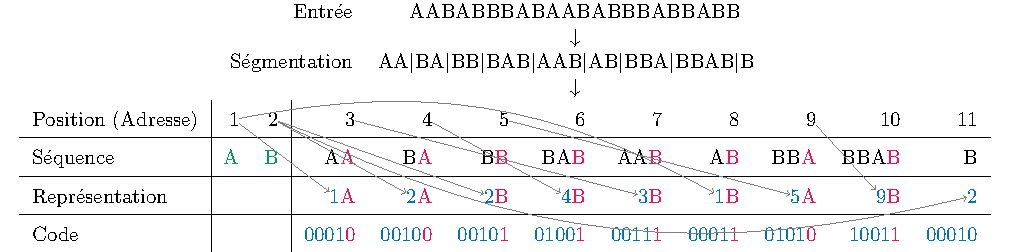
\includegraphics[width=\columnwidth]{drwg_0.pdf}
\end{figure}




\section{Transmission sans-fil}
\subsection{Formule de Friis}
Dans un cas idéal, sans trajets multiples
$$\frac{P_r}{P_t}=G_tG_r\left(\frac{\lambda}{4\pi R}\right)^2$$
en \si{\deci\bel} : 
$$\underbrace{(P_r)_{\si{\deci\bel}}-(P_t)_{\si{\deci\bel}}}_{Att_{\si{\deci\bel}}}=(G_t)_{\si{\deci\bel}}+(G_r)_{\si{\deci\bel}}+20\log_{10}\left(\frac{\lambda}{4\pi R}\right)$$
$$(x)_{\si{\deci\bel}}=10\log_{10}(x)$$
A noter que la puissance de 2 a été enlevée et le $10\log$ remplacé par $20\log$
\subsection{Capacité du canal et efficacité spectrale}
$$\frac{C}{B}=\log_2\left(1+\frac{S}{N}\right)=\log_2\left(1+\frac{E_bR}{N_0B}\right)$$
La limite est donnée par
$$\frac{E_b}{N_0}=B\frac{2^{\frac{C}{B}-1}}{R}$$
\subsection{Autres}
$$\SI{1}{\watt}=\SI{30}{\deci\bel m}$$
\subfile{codage_canal}






\end{multicols}
\end{document}